\chapter{Strømforsyning}
Ud fra kravspecifikation skal delmodulerne (SM og VBTE) kunne drives fra en 24V AC/DC forsynings kilde. Selve modulerne er designet til 12V DC og 5V DC forsyningsspændringer , der designes derfor en strømforsyning der regulere spændingen så den kan levere 12V 1A og 5V 0,5A.  

\section{Overordnet design}
I dette afsnit beskrives og vises det overordnede hardware blokdiagram over strømforsyningen samt beskrivelse signaler.

\begin{figure}[H]
\centering
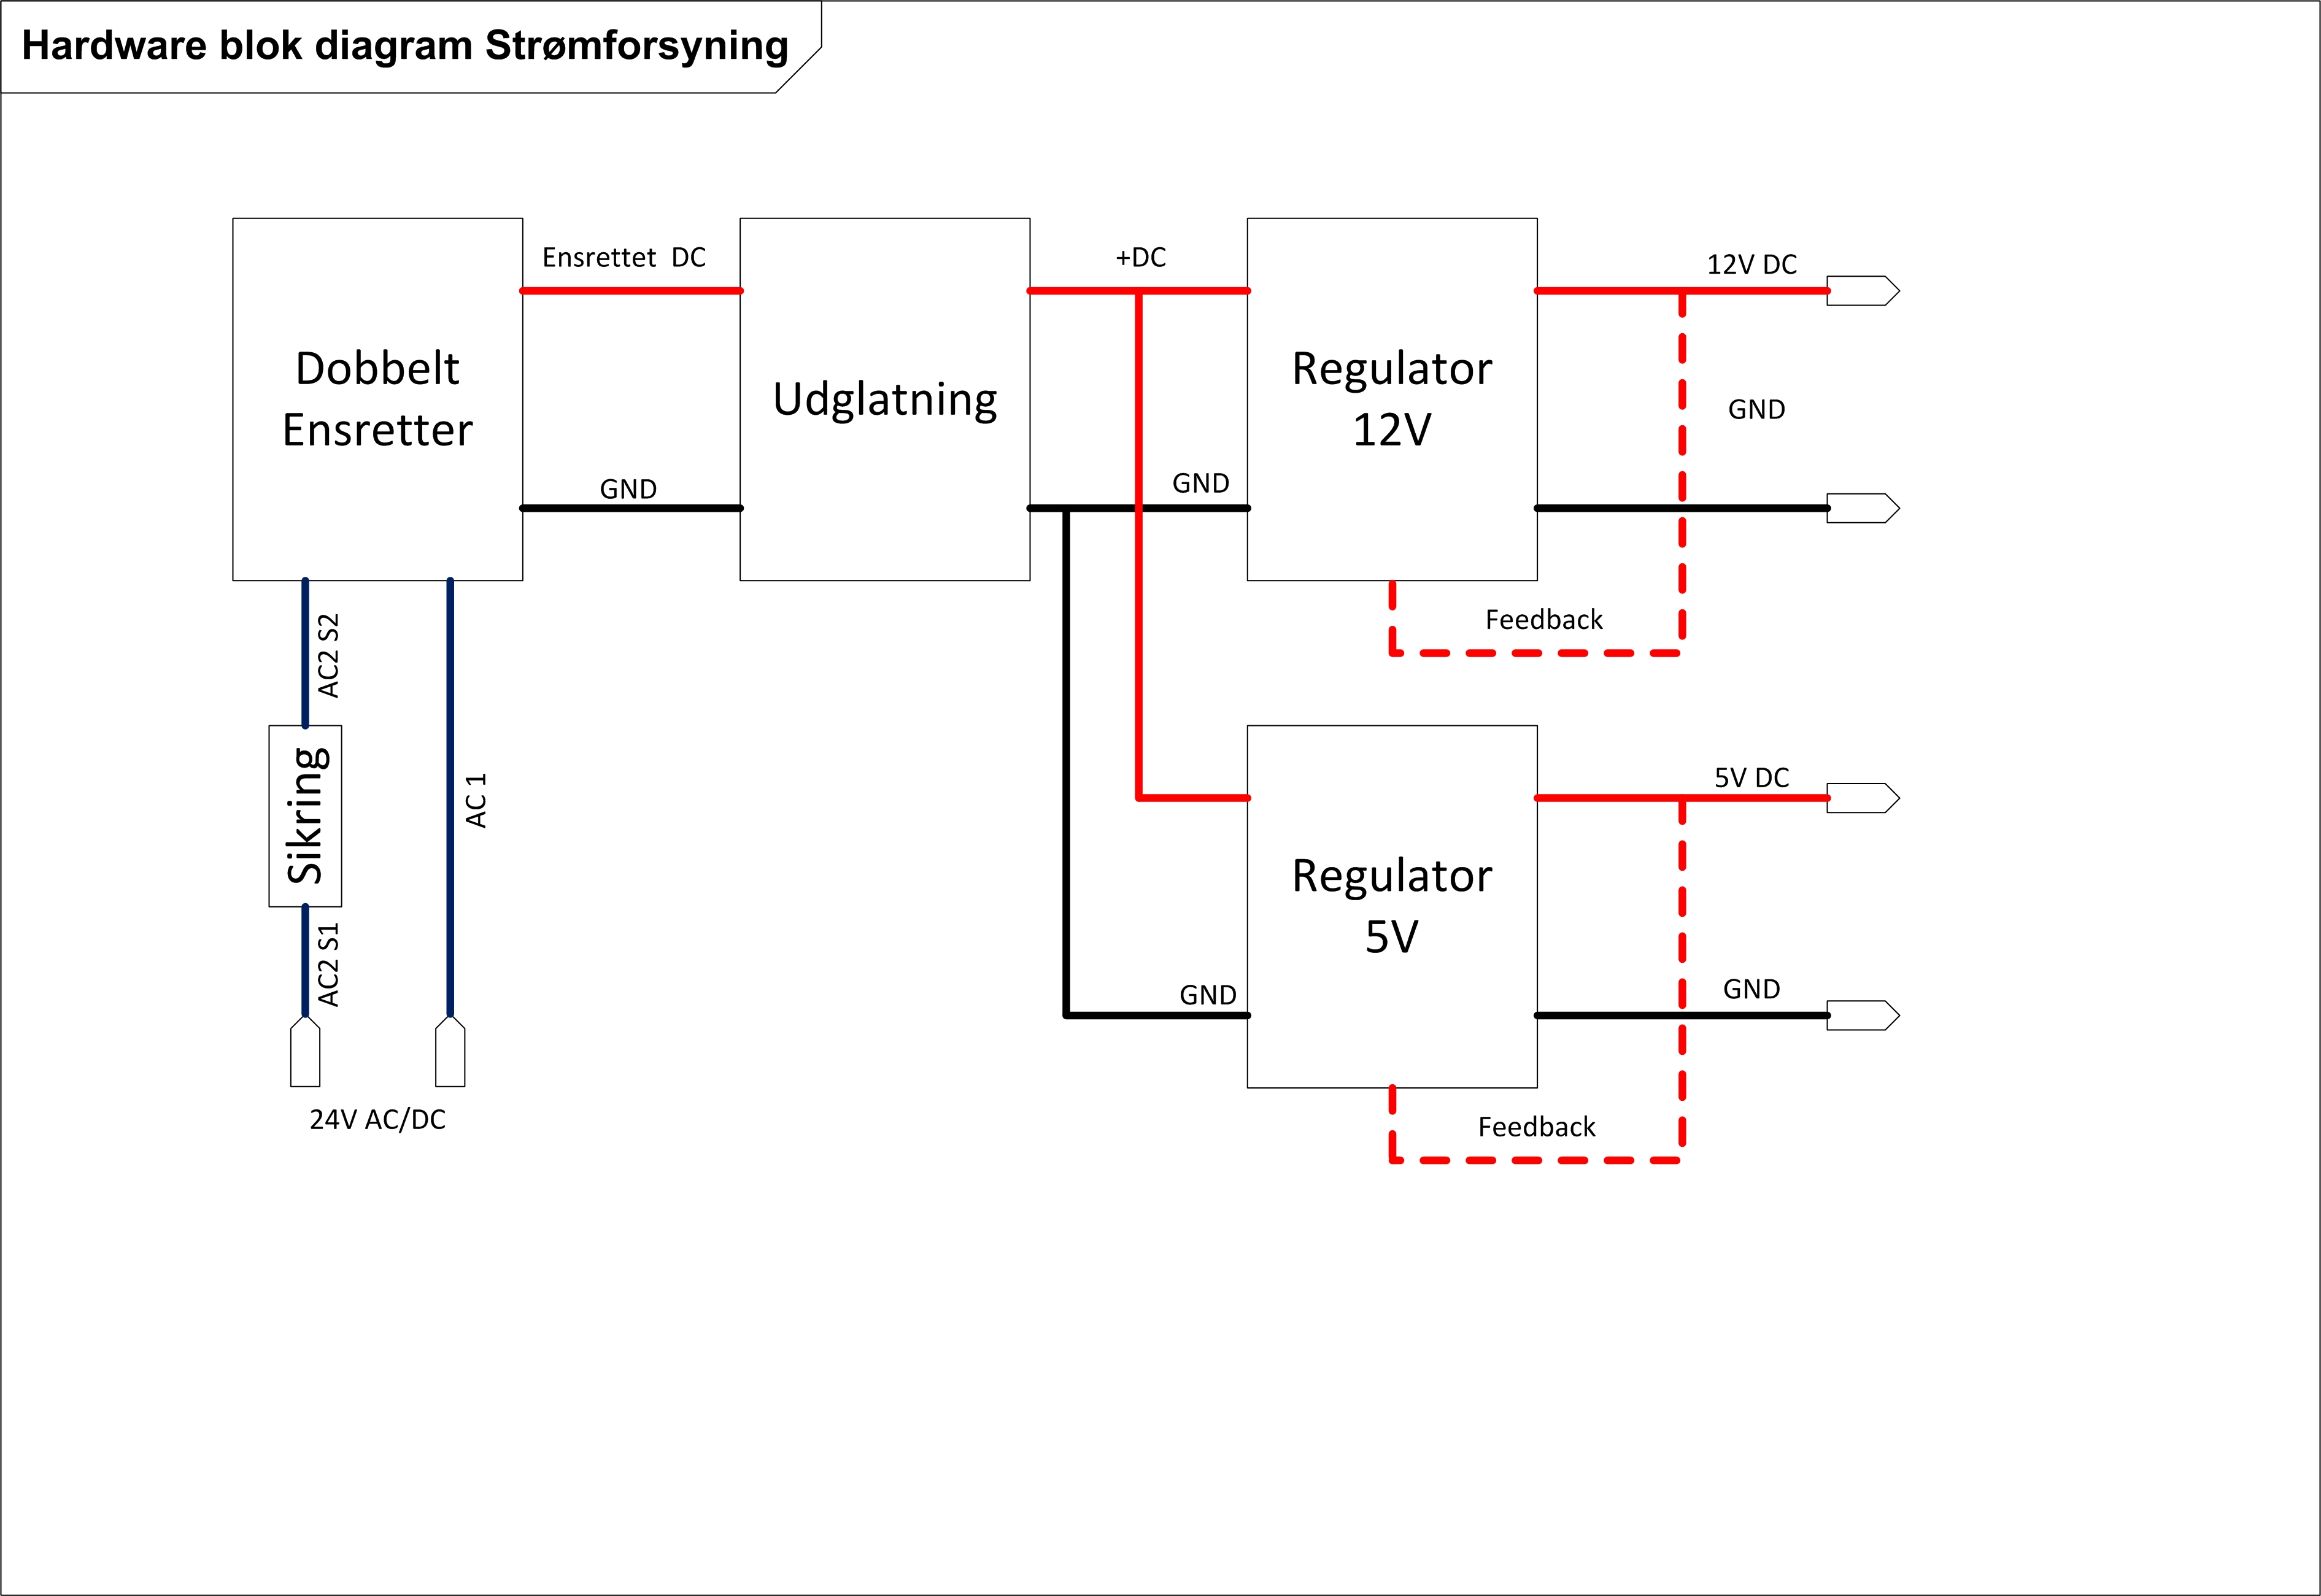
\includegraphics[width=1\textwidth]{billeder/PowerSupplyBlok}
\caption{Overordnet blokdiagram for strømforsyning}
\label{fig:PowerSubbly Blok}
\end{figure}
\newpage
\subsection{Blokke}
Nedenfor beskrives de enkelte blokke illustreret på \textit{Figur~\ref{fig:PowerSubbly Blok}}
\subsubsection{Sikring}
Sikringen beskytter forsyningskilde, hvis der bliver for stor belastning på strømforsyningen
\subsubsection{Dobbelt ensretter}
Ensretter AC eller DC spændingen fra forsyningskilden.
\subsubsection{Udglatning}
Udglatter det ensrettet signal til en stabil positiv DC. 
\subsubsection{Regulator 12V}
Regulere den ensrettet DC ned til 12V DC.
\subsubsection{Regulator 5V}
Regulere den ensrettet DC ned til 5V DC.
\newpage
\section{Nedbrydning af blokke}
For at gøre designet af de forskellige blokke mere overskuelig nedbrydes de enkle blokke fra det overordnede blokdiagram.
\subsection{Sikring}
\begin{figure}[H]
\centering
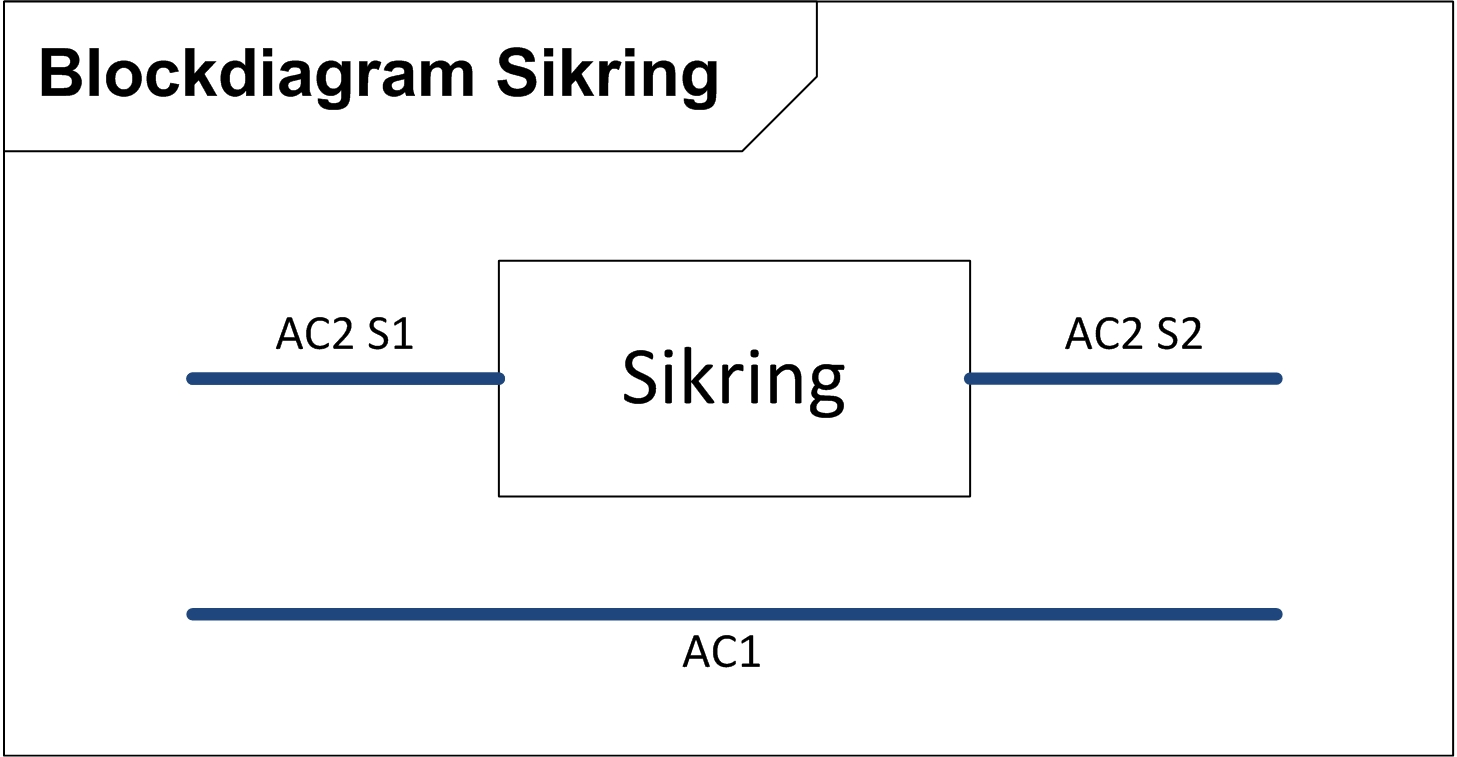
\includegraphics[scale=1]{billeder/SikringsBlok}
\caption{Blokdiagram for Sikrings blok}
\label{fig:SikringsBlok}
\end{figure}
\subsubsection{Signalbeskrivelser}
I tabellen beskrives de interne signaler
\begin{table}[H]
\begin{tabular}{|p{3cm}|p{3cm}|p{3cm}|p{4.5cm}|} \hline
\cellcolor[gray]{0.85}Signal navn& \cellcolor[gray]{0.85}Type &\cellcolor[gray]{0.85}Spænding&\cellcolor[gray]{0.85}Beskrivelse\\ \hline
AC/DC\_1 S1 & Analog  & 24V AC / 24V DC & Indgangsspænding fra spændingskilde inden sikring.\\  \hline
AC/DC\_1 S2  & Analog & 24V AC / 24V DC & Indgangsspænding fra spændingskilde efter sikring. \\  \hline
AC/DC\_2 & Analog & 0V AC / 0V DC & 0V AC eller 0V DC fra spændingskilde.\\  \hline
\end{tabular}
\caption{Tabel over signaler i Sikringsblokken}
\label{table:SikringSignaler}
\end{table}
